\documentclass{ieeeaccess}
\usepackage{cite}
\usepackage{amsmath,amssymb,amsfonts}
%\usepackage{algorithm}
\usepackage{algorithmic}
\usepackage[ruled, vlined, linesnumbered]{algorithm2e}
\usepackage{graphicx}
\usepackage{textcomp}

\usepackage{enumitem}

%Please add the following packages if necessary:
\usepackage{booktabs, multirow} % for borders and merged ranges
\usepackage{soul}% for underlines
\usepackage[table]{xcolor} % for cell colors
\usepackage{changepage,threeparttable} % for wide tables

\usepackage[commentmarkup=footnote,final]{changes} % Add changes for correction in text. USE THIS FOR FINAL VERSION
%\usepackage[commentmarkup=footnote]{changes} % Add changes for correction in text. USE THIS FOR REVIEW


\newcommand\Fig[1]{\textbf{Fig.}~\ref{#1}}
\newcommand\fig[1]{\textbf{Fig.}~\ref{#1}}
\newcommand\Tab[1]{\textbf{Tab.}~\ref{#1}}
\newcommand\tab[1]{\textbf{Tab.}~\ref{#1}}
\newcommand\Equ[1]{\textbf{Eq.}~(\ref{#1})}
\newcommand\equ[1]{\textbf{Eq.}~(\ref{#1})}
\newcommand\Sect[1]{\textbf{Sec.}~\ref{#1}}
\newcommand\sect[1]{\textbf{Sec.}~\ref{#1}}
\newcommand\Refs[1]{\textbf{Ref.}~\cite{#1}}
\newcommand\refs[1]{\textbf{Ref.}~\cite{#1}}


\newcommand\todo[1]{\textbf{(TODO: {#1}})\\}

% To highlight "review"
\newcommand\REVIEW[1]{\hl{#1}}
%To remove highlight
%\newcommand\REVIEW[1]{{#1}}

\begin{document}
\history{Date of publication xxxx 00, 0000, date of current version xxxx 00, 0000.}
\doi{10.1109/ACCESS.2017.DOI}


\begin{abstract}
In this article, we present a design exploration framework for floating-point convolutional neural networks (CNNs) acceleration on low-power, resource-limited embedded FPGAs targeting IoT sensor data analytic applications. We propose a scalable hardware architecture with customizable tensor processors (TPs) integrated with TensorFlow Lite. The implemented hardware optimization realizes hybrid custom floating-point and logarithmic dot-product approximation. This approach accelerates computation, reduces energy consumption and resource utilization while maintaining inference accuracy. Experimental results on MiniZed (XC7Z007S) and Zybo (XC7Z010) demonstrate peak acceleration and power efficiency of 105X and 5.5 GFLOP/s/W, respectively.
\end{abstract}

\begin{IEEEkeywords}
Artificial intelligence, convolutional neural networks, depthwise separable convolution, hardware accelerator, TensorFlow Lite, embedded systems, FPGA, custom floating-point, logarithmic computation, approximate computing
\end{IEEEkeywords}


\section{Introduction}
\label{sec:introduction}
%%% General intro
\PARstart{A}{rtificial} Intelligence (AI) is increasingly attracting the interest of industry and academia; in particular,  Artificial Neural Networks (ANNs). Historically, ANNs can be classified into three different generations \cite{Design_Exploration_SbS_Trans20}: the first one is represented by the classical McCulloch and Pitts neuron model using discrete binary values as outputs; the second one is represented by more complex architectures as Multi-Layer Perceptrons and Convolutional Neural Networks (CNN) using continuous activation functions; while the third generation is represented by Spiking Neural Networks (SNNs) using spikes as means for information exchange between groups of neurons. Although the AI field is currently dominated by Deep Neural Networks (DNN) from the second generation, nowadays the SNNs belonging to the third generation are receiving considerable attention \cite{Spinnaker_Trans13,ernst2007efficient,Design_Exploration_SbS_Trans20, SNN_Survey_Trans19} due to their advantages in terms of robustness and the
potential to achieve a power efficiency close to that of the human
brain (see section~\ref{sec:sbs} for more details).

%%% SbS intro
Among the family of SNNs, the SbS neural network \cite{ernst2007efficient} is inspired by the natural computing of the mammalian brain, being a biologically plausible approach although with less complexity than other SNNs. The SbS model differs fundamentally from conventional ANNs since (a) the building block of the network are inference populations (IP) which are an optimized generative representation with non-negative values, (b) time progresses from one spike to the next, preserving the property of stochastically firing neurons, and (c) a network has only a small number of parameters, which is an advantageous stochastic version of Non-Negative Matrix Factorization (NNMF), which is noise-robust and easy to handle. In regard to biological realism and computational effort to simulate neural networks, these properties place the SbS network in between non-spiking NN and stochastically spiking NN \cite{rotermund2019Backpropagation}.

%%%%%%% Problem statement
In \cite{nevarez2020accelerator} we presented an accelerator framework which allows design exploration of dedicated hardware for SbS network computation in embedded systems. However, the high computational cost and memory footprint are the fundamental constrains of such resource-limited devices. Using logarithmic quantization have demonstrated higher classification accuracy than fixed-point at low resolutions; however, this alternative requires quantization-aware training methods. As an alternative, we use approximate computing as a design paradigm to leverage the intrinsic resilience of SbS networks to execute computations approximately, leading to higher efficiency and performance enhancement.

%%%%%%% Contributions
In this paper, we present a hardware architecture for non-quantized SbS network simulations based on approximate dot-product computation using hybrid custom floating-point and logarithmic number representation. The proposed hardware module for dot-product computation has the following main characteristics, (1) to increase computational throughput, the element-wise multiplication is done by adding integer exponents as well as accumulation is done by adding denormalized integer products, (2) to reduce memory footprint, the synaptic weight vector uses either reduced custom floating-point or logarithmic representation, and (3) to preserve inference accuracy, the neuron vector uses either standard or reduced custom floating-point representation. On the proposed architecture, we evaluate computational latency, accuracy degradation, noise robustness, resource utilization and power dissipation.

The rest of the paper is organized as follows. Section~\ref{sec:related_work} covers the related work; Section~\ref{sec:background} introduces the background; Section~\ref{sec:system_design} describes the system design; Section~\ref{sec:experimental_results} presents the experimental results; Section~\ref{sec:conclusions} concludes the paper.


To promote the research on SbS, the entire framework is made available to the public as an open-source project at http://www.ids.uni-bremen.de/sbs-framework.html


\section{Related work}
\label{sec:related_work}
%%%%%%%%%%%%%%%%%%%%%%%%%%%%%%%%%%%%%%%%%%%%%%%%%%%%%%
\subsection{Approximate computing in neural networks}
Approximate computing has been used in a wide range of applications to increase the computational efficiency in hardware\cite{han2013approximate}. For neural network applications, two main approximation strategies are used, namely network compression and classical approximate computing\cite{bouvier2019spiking}.

\subsubsection{Network compression}
Researchers focusing on embedded applications started lowering the precision of weights and activation maps to shrink the memory footprint of the large number of parameters representing ANNs, a method known as network compression or quantization. This practice takes advantage of the intrinsic error-tolerance of neural networks, as well as their ability to compensate for approximation while training. In this way, reduced bit precision causes a small accuracy loss \cite{courbariaux2015binaryconnect, han2015deep, hubara2017quantized, rastegari2016xnor}.

In hardware development, weight quantization (WQ) has shown up to $2\times$ improvement in energy consumption with an accuracy degradation of less than $1\%$ \cite{moons20160, whatmough201714}. Some advanced quantization methods yield to binary neural networks (BNNs) allowing the use of XNORs instead of the conventional costly multiply-accumulate circuits (MACs) \cite{rastegari2016xnor}. In \cite{sun2018xnor}, Sun et al. report an accuracy of $98.43\%$ on handwritten digit classification with a simple BNN. Hence, quantization is a powerful tool for improving the energy efficiency and memory requirements of ANN accelerators, with limited accuracy degradation.

In addition to quantization, network pruning reduces the model size by removing structural portions of the parameters and its associated computations \cite{lecun1989optimal,hassibi1992second}. This method has been identified as an effective technique to improve the efficiency of DNN for applications with limited computational budget\cite{molchanov2016pruning,li2016pruning, liu2018rethinking}.

These methods can be used for SNNs as well. In \cite{rathi2018stdp}, Rathi et al. report up to $3.1\times$ improvement in energy consumption with an accuracy loss of around $3\%$. Weight quantization allows the designer to realize a trade-off between the accuracy of the SNN application and efficiency of resources. Approximate computing can also be applied at the neuron level, where irrelevant units are deactivated to reduce the computation cost of the SNNs \cite{sen2017approximate}. This computation skipping can be applied randomly on synapses, training ANNs with stochastic synapses improves generalization, resulting in a better accuracy\cite{srivastava2014dropout, wan2013regularization}. Such methods are compatible with SNNs and have been tested both during training \cite{neftci2016stochastic, srinivasan2016magnetic} and operation \cite{buesing2011neural}, and even to define the connectivity between layers \cite{bellec2017deep, chen20184096}. Implementations of spiking neuromorphic systems in FPGA \cite{sheik2016synaptic} and hardware \cite{jerry2017ultra} demonstrated that synaptic stochasticity allows to increase the final accuracy of the networks while reducing memory footprint.

Quantization is therefore a powerful technique to improve energy efficiency and memory requirements of ANN and SNN accelerators, with small accuracy degradation. However, this approach requires quantization-aware training methods that, in some cases, are problematic or even inaccessible, particularly in emerging deep SNN algorithms\cite{zhang2018survey}.

\subsubsection{Classical approximate computing}
This approach consists of designing processing elements that approximate their computation by employing modified algorithmic logic units \cite{han2013approximate}. In \cite{kim2013energy}, Kim et al. have shown SNNs using carry skip adders achieving $2.4\times$ latency enhancement and $43\%$ more energy efficiency, with an accuracy degradation of 0.97\% on a handwritten digit classification task. Therefore, approximate computing provides important enhancement in energy efficiency and processing speed.

However, as the complexity of the dataset increases, as well as the depth of the network topology, such as ResNet \cite{he2016deep} on ImageNet \cite{russakovsky2015imagenet}, the accuracy degradation becomes more important and may not be negligible anymore \cite{rastegari2016xnor}, especially for critical applications such as autonomous driving. Therefore, it is not certain that network compression techniques and approximate computing are suitable for \replaced{all}{some} applications.

\subsection{Spike-by-Spike neural networks accelerators}
Recently, Rotermund et al.\ demonstrated the feasibility of a neuromorphic SbS IP on a Xilinx Virtex 6 FPGA \cite{rotermund2018massively}. It provides a massively parallel architecture, optimized to reduce memory access and suitable for ASIC implementations. Nonetheless, this design is considerably resource-demanding if implemented as a full SbS network in today's embedded technology.

In \added{Ref.~}\cite{nevarez2020accelerator}, we presented a cross-platform accelerator framework for design exploration and testing of fully functional SbS network models in embedded systems. As a hardware/software (HW/SW) co-design solution, this framework offers a comprehensive high level embedded software API that allows the construction of scalable sequential SbS networks with configurable hardware acceleration.
\REVIEW
{However, this design works entirely with standard floating-point arithmetic (IEEE 754). This represents a large memory footprint and inadequate computational cost for error resilient applications on resource-limited devices.
}
 In this article, we will use this design exploration framework to investigate approximate computing for efficient deployment of deep SbS networks on resource-limited devices.
%%%%%%%%%%%%%%%%%%%%%%%%%%%%%%%%%%%%%%%%%%%%%%%%%%%%%%
\section{Background}
\label{sec:background}
\subsection{Conv2D tensor operation}
The \emph{Conv2D} tensor operation is described in \Equ{eq:conv2D}, where $h$ is the input feature map, $W$ is the convolution kernel (known as filter), and $b$ is the bias for the output feature map\cite{goodfellow2016deep}. We denote \emph{Conv} as \emph{Conv2D} operator.
\begin{eqnarray} \label{eq:conv2D}
Conv\left(W,h\right)_{i,j,o}=\sum_{k,l,m}^{K,L,M} h_{(i+k,j+l,m)} W_{(o,k,l,m)}+b_{o}
\end{eqnarray} 	
\subsection{DepthwiseConv2D tensor operation}
The \emph{DepthwiseConv2D} tensor operation is described in \Equ{eq:dconv2D}, where $h$ is the input feature map, $W$ is the convolution kernel (known as filter), and $b$ is the bias for the output feature map. We denote \emph{DConv} as \emph{DepthwiseConv2D} operator.
\begin{eqnarray} \label{eq:dconv2D}
DConv\left(W,h\right)_{i,j,n}=\sum_{k,l}^{K,L} h_{(i+k,j+l,n)} W_{(k,l,n)}+b_{n}
\end{eqnarray}
\section{System Design}
\label{sec:system_design}

\REVIEW{
	In this section, we revise the system design of \mbox{\cite{nevarez2020accelerator}}. In Ref. \mbox{\cite{nevarez2020accelerator}}, we presented a scalable hardware architecture composed of generic homogeneous accelerator units (AUs) using standard floating-point arithmetic (IEEE 754). This approach represents an overhead for error-resilient applications due to the elevated memory footprint and computational cost. Furthermore, this architecture does not implement stationary synaptic weight matrix in the hardware AUs, resulting in heavy data movement and longer computational latency.
	
	In this publication, we present an enhanced hardware architecture composed of specialized heterogeneous processing units (PUs) with hybrid custom floating-point and logarithmic dot-product approximation. This approach represents an advantageous design for error-resilient applications in resource-constrained devices due to the reduced computational costs and memory footprint. Furthermore, the proposed approach allows the implementation of stationary synaptic weight matrices. These novelties result in an improved overall system design.
	}

Regarding the software architecture, this is structured as a
layered object-oriented application framework written in the C programming language. This offers a comprehensive high level embedded software application programming interface (API) that allows the construction of scalable sequential SbS networks with configurable hardware acceleration. Conceptually this design is modular, reusable, and extensible. The overall structure is depicted in \fig{fig:sw_stack}.

\begin{figure}[t!]
	\centering
	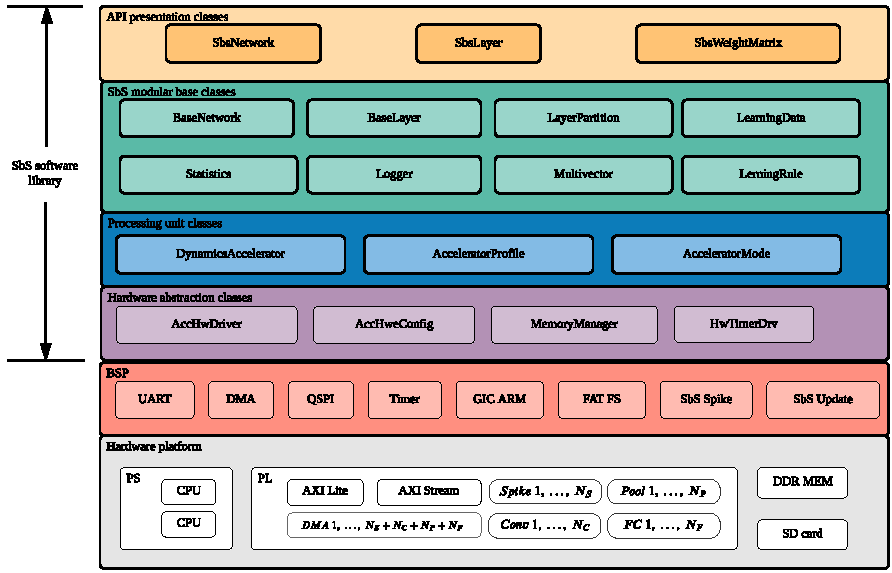
\includegraphics[width=0.5\textwidth]{../figures/sbs_software_component.pdf}
	\caption{System-level overview of the embedded software architecture.}
	\label{fig:sw_stack}
\end{figure}

\subsection{Hardware architecture} \label{Hardware_architecture}
As a hardware/software co-design, the system architecture is an embedded CPU+FPGA-based platform, where the acceleration of SbS network computation is based on asynchronous\footnote{The system is synchronous at the circuit level, but the execution is asynchronous in terms of jobs.} execution \replaced{in}{of} parallel heterogeneous processing units: \emph{Spike} (input layer), \emph{Conv} (convolution), \emph{Pool} (pooling), and \emph{FC} (fully connected). \fig{fig:hw_sbs} illustrates the system \replaced{hardware architecture}{overview} as a scalable structure. For hardware configuration, each PU uses AXI-Lite interface. For data transfer, each PU uses AXI-Stream interfaces via Direct Memory Access (DMA) allowing data movement with high transfer rate. Each PU asserts an interrupt flag once the job or transaction is complete. This interrupt event is handled by the embedded CPU to collect results and start a new transaction.

The hardware architecture can resize its resource utilization by changing the number of PUs instances \REVIEW{prior to the hardware synthesis}, this provides scalability with a good trade-off between area and throughput. The dedicated PUs for \emph{Conv} and \emph{FC} implement the proposed dot-product approximation as a system component. The PUs are written in C using Vivado HLS (High-Level Synthesis) tool. In this publication, we illustrate the integration of the approximate dot-product component on the \emph{Conv} processing unit.

\begin{figure}[t!]
	\centering
	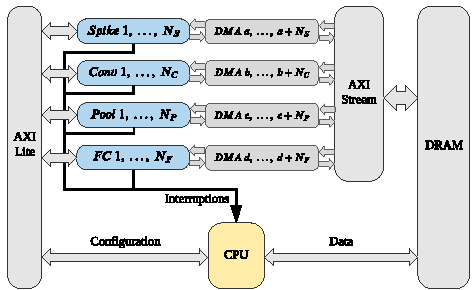
\includegraphics[width=0.5\textwidth]{../figures/sbs_hw.pdf}
	\caption{System-level hardware architecture with scalable number of heterogeneous PUs: \emph{Spike}, \emph{Conv}, \emph{Pool}, and \emph{FC}}
	\label{fig:hw_sbs}
\end{figure}

\subsection{Conv processing unit}
This hardware module computes the IP dynamics defined by \equ{eq:sbs_update} and offers two modes of operation: \emph{configuration} and \emph{computation}.

\subsubsection{Configuration mode}
In this mode of operation, the PU receives and stores in on-chip memory (BRAM) the parameters to compute the IP dynamics: $\epsilon$ as the epsilon, $N$ as the length of $\vec{h}_\mu\in\mathbb{R}^{N}$, $K\in\mathbb{N}$ as the size of the convolution kernel, and $H\in\mathbb{N}$ as the number of IPs to process per transaction. $H$ is the number of IPs forming a layer or a partition.

Additionally, the processing unit also stores in on-chip memory (BRAM) the synaptic weight matrix using a number representation with a reduced memory footprint. Fundamentally, the synaptic weight matrix is defined by $W\in\mathbb{R}^{K\times K\times M\times N}$ with $0\le W(s_t|j)\le1$ and $\sum_{j=0}^{N-1}W(s_t|j)=1$ \cite{rotermund2019Backpropagation}. Hence, $W$ employs only positive normalized real numbers. Therefore, $W$ is deployed using a reduced floating-point or logarithmic representation as follows:

\begin{itemize}
	\item{Custom floating-point representation}.
	In this case, $W$ is deployed with a reduced floating-point representation using the user defined bit-width for the exponent and for the mantissa. For example, 4-bit exponent, 1-bit mantissa; as a result: 5-bit custom floating-point.
	\item{Logarithmic representation}.
	In this case, the synaptic weight matrix is $W\in\mathbb{N}^{K\times K\times M\times N}$ with positive natural numbers. Since $0\le W(s_t|j)\le1$ and $\sum_{j=0}^{N-1}W(s_t|j)=1$, $W$ has only negative values in the logarithmic domain. Hence, the sign bit is omitted, and the values are represented in its positive form. Therefore, $W$ is deployed with a representation using the necessary bit-width for the exponent according to the given application. For example, 4-bit exponent.
\end{itemize}

In order to deploy different SbS network models, the \emph{Conv} processing units can be configured with different synaptic weight matrices and parameters as required through the embedded software.

\subsubsection{Computation mode}
In this mode of operation, the PU executes a transaction to process a group of IPs using the previously given parameters and synaptic weight matrix. This process operates in six stages as shown in \fig{fig:hw_conv}. In the first two stages, the PU receives $\vec{h}_\mu\in\mathbb{R}^{N}$, then the PU calculates the emitted spike, and stores it in $S^{new}\in\mathbb{N}^{H}$ (output spike vector). From the third to the fifth stage, the PU receives $S_t\in\mathbb{N}^{K\times K}$ (input spike matrix), then it computes the update dynamics, and then it dispatches $\vec{h}_\mu^{new}\in\mathbb{R}^{N}$ (updated IP). This process repeats for $H$ number of loops (for each IP of the layer or partition). Finally, the $S^{new}$ is dispatched.

The computation of the update dynamics (see \fig{fig:hw_conv}(d)) operates in two modular stages: \emph{dot-product} and \emph{neuron update}. First, the \emph{dot-product} module calculates the sum of pairwise products of $\vec{h}_{\mu}$ and $\vec{W}(s_t)$, while storing each pairwise product as intermediate results. Subsequently, the \emph{neuron update} module calculates \equ{eq:sbs_update} reusing previous results and parameters.


The calculation of the dot-product of \equ{eq:sbs_update} represents a considerable computational cost using standard floating-point in non-quantized network models. Fortunately, the pair product of $h_{\mu}(j)$ and $W(s_t|j)$ was defined by us as an approximable factor in the dot-product of \equ{eq:sbs_update}. In the following section, we focus on an optimized dot-product hardware design based on approximate computing.


\begin{figure}[t!]
	\centering
	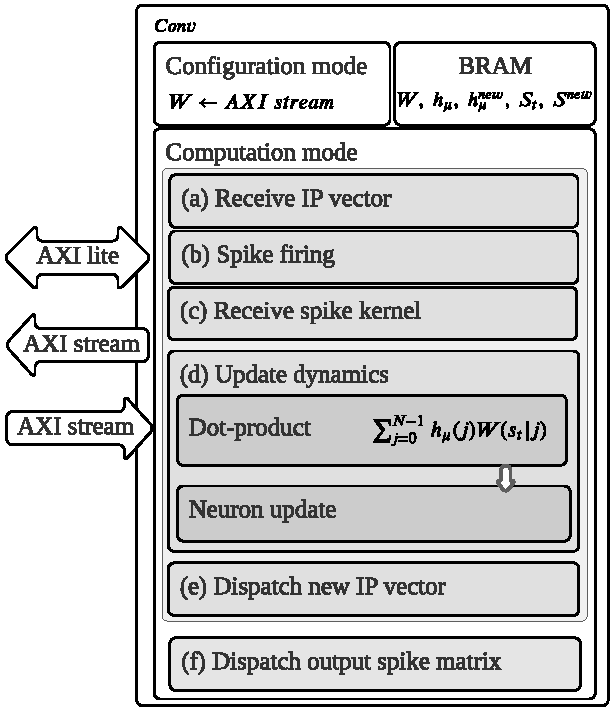
\includegraphics[width=0.5\textwidth]{../figures/sbs_conv.pdf}
	\caption{The \emph{Conv} processing unit and its six stages: (a) receive IP vector, (b) spike firing, (c) receive spike kernel, (d) update dynamics, (e) dispatch new IP vector, (f) dispatch output spike matrix.}
	\label{fig:hw_conv}
\end{figure}

\subsection{dot-product hardware module}
This dot-product hardware module is part of an application-specific architecture optimized to approximate the dot-product of arbitrary length, see \equ{eq:dot_product}. For quality configurability, we parameterized the mantissa bit-width of $\vec{W}(s_t)$, which provides a tunable trade-off between resource utilization and QoR. Since the lower-order bits have smaller significance than the higher-order bits, removing them may have only a minor impact on QoR. We designate this as hybrid custom floating-point approximation \REVIEW{(see {\fig{fig:product_unit_bitwidth}}(a))}.

\begin{eqnarray} \label{eq:dot_product}
r_{\mu}\left(s_t\right)=\sum_{j=0}^{N-1}h_{\mu}(j)W(s_t|j)
\end{eqnarray}

Further on, we remove the mantissa bits completely in order to use only the exponent of a floating-point representation. Hence, the worst-case quality and yet the most efficient configuration becomes a logarithmic representation. Consequently, this structure leads to advantageous architectural optimizations using only adders and barrel shifters for dot-product approximation in hardware. We designate this as hybrid logarithmic approximation \REVIEW{(see {\fig{fig:product_unit_bitwidth}}(b))}.

\REVIEW{
In order to determine the required bit-width for the number representation, we use {\equ{eq:exp_max}}, {\equ{eq:bits_exp}}, and {\equ{eq:bits_bitwidth}}. Where {\equ{eq:exp_max}} obtains the smallest entry value from the synaptic weight matrix, {\equ{eq:bits_exp}} obtains the bit-width to represent the integer exponent of the smallest synaptic weight value, and {\equ{eq:bits_bitwidth}} obtains the total bit-width required for the number representation of the input synaptic weight vector $\vec{W}(s_t)$. The total bit-width incorporates both exponent and mantissa bit-widths (see {\fig{fig:product_unit_bitwidth}}). $N_M$ denotes the mantissa bit-width, this is a knob parameter that is tuned by the designer to trade-off between resource utilization and QoR.
}

\begin{eqnarray} \label{eq:exp_max}
E_{\min}=\log _2(\min_{\forall i}(W(i)))
\end{eqnarray}

\begin{eqnarray} \label{eq:bits_exp}
N_E=\lceil\log_2(|E_{\min}|)\rceil
\end{eqnarray}

\begin{eqnarray} \label{eq:bits_bitwidth}
N_W=N_E + N_M
\end{eqnarray}

\begin{figure}
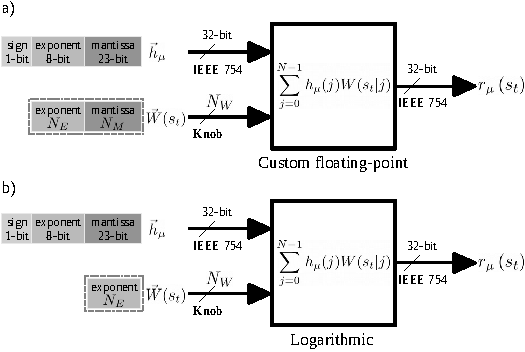
\includegraphics[width=\columnwidth]{../figures/dot-product_unit_bitwidth.pdf}
\caption{Dot-product hardware module with (a) hybrid custom floating-point approximation, and (b) hybrid logarithmic approximation.}
\label{fig:product_unit_bitwidth}
\end{figure}

In this section, we will present three pipelined hardware modules with standard floating-point (IEEE 754) computation, hybrid custom floating-point approximation, and hybrid logarithmic approximation.

\subsubsection{Dot-product with standard floating-point computation}
 The hardware module to calculate the dot-product with standard floating-point computation is shown in \fig{fig:dot_product_float}. This diagram presents the hardware blocks and their clock cycle schedule. This module loads both $h_\mu(j)$ and $W(s|j)$ from BRAM, then the PU executes the pairwise product (\fig{fig:dot_product_float}(c)) and accumulation (\fig{fig:dot_product_float}(d)). The intermediate results of $h_\mu(j) W(s_t|j)$ are stored in BRAM for reuse in the neuron update. The latency in clock cycles of this hardware module is defined by \equ{eq:dot_standard_float_latency}, where $N$ is the dot-product length. This latency equation is obtained from the general pipelined hardware latency formula: $L=\left(N-1\right)II+IL$, where $II$ is the initiation interval (\fig{fig:dot_product_float}(a)), and $IL$ is the iteration latency (\fig{fig:dot_product_float}(b)). Both $II$ and $IL$ are obtained from the high-level synthesis analysis. The equation for the latency with standard 32-bit floating-point is:
 \begin{eqnarray} \label{eq:dot_standard_float_latency}
 L_{f32}=10N+9
 \end{eqnarray}
 
In this design, the high level synthesis tool infers computational blocks with considerable latency cost for standard floating-point. In the case of floating-point multiplication (\fig{fig:dot_product_float}(c)), the synthesis infers a hardware block with a latency cost of 5 clock cycles. Theoretically, this block would handle exponents addition, mantissas multiplication, and mantissa correction if needed. Moreover, in the case of floating-point addition (\fig{fig:dot_product_float}(d)), the synthesis infers a hardware block with a latency cost of 9 clock cycles. Seemingly, this block would handle mantissas alignment, addition, and correction if needed. Therefore, the use of standard floating-point in high-level synthesis results in high computational cost, which represents unnecessary overhead in error-tolerant applications.


\begin{figure}[t!]
	\centering
	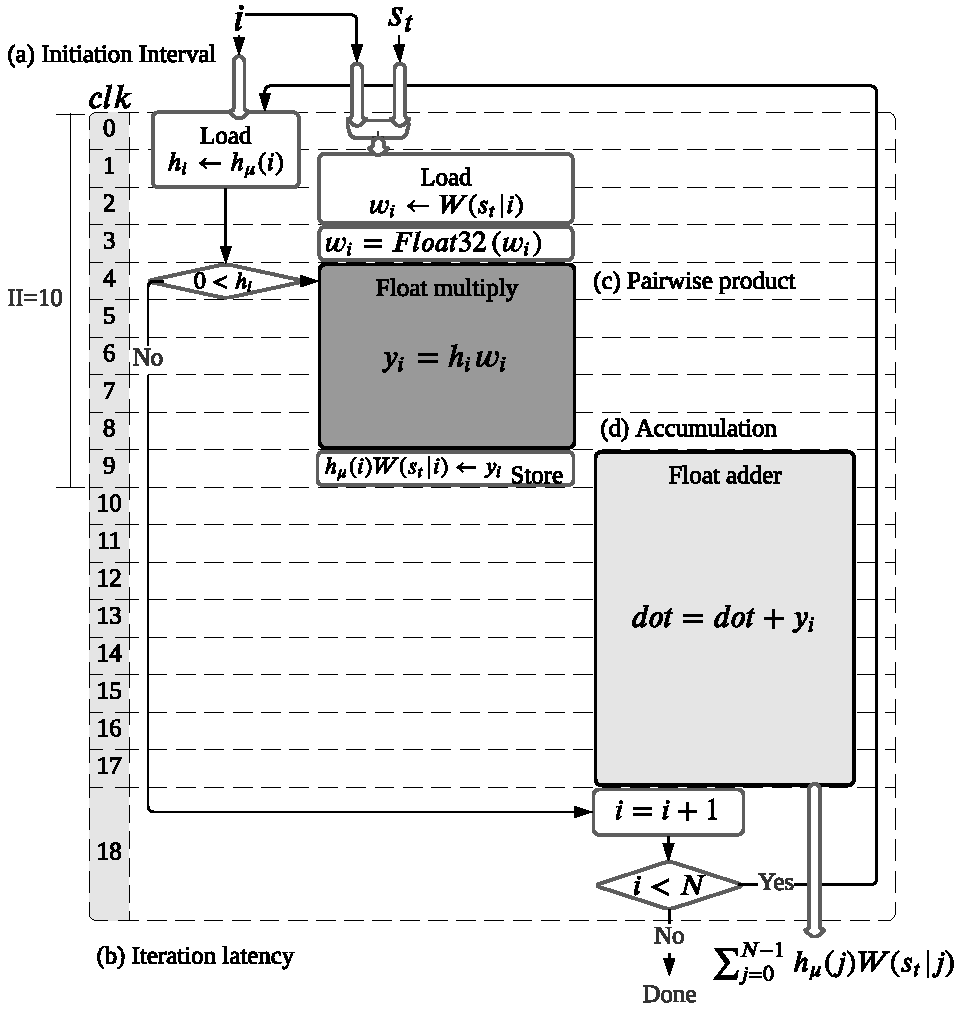
\includegraphics[width=0.5\textwidth]{../figures/dot_product_float.pdf}
	\caption{Dot-product hardware module with standard floating-point (IEEE 754) computation, (a) exhibits the initiation interval of 10 clock cycles, (b) presents the iteration latency of 19 clock cycles, (c) shows the pairwise product block in dark-gray, and (d) illustrates the accumulation block in light-gray.}
	\label{fig:dot_product_float}
\end{figure}

\subsubsection{Dot-product with hybrid custom floating-point and logarithmic approximation}
 The hardware module to calculate dot-product with hybrid custom floating-point approximation is shown in \fig{fig:dot_product_custom}. In this design, $h_\mu(j)$ uses standard 32-bit floating-point number representation, and $W(s|j)$ uses a positive reduced custom floating-point number representation, where the mantissa bit width is the quality configurability knob. This parameter is tuned by the designer to trade-off between QoR and resource utilization, thus, energy consumption.
 
 As the most efficient setup and yet the worst-case quality configuration, by completely truncating the mantissa of $W(s|j)$ leads to a slightly different hardware architecture using only adders and shifters, which computes the dot-product with hybrid logarithmic approximation. This is shown in \fig{fig:dot_product_log}.
 
Additionally, the exponent bit-width of $W(s|j)$ is a design parameter for efficient resource utilization and it is defined based on the application or deployment needs.
 
 The hybrid custom floating-point and logarithmic approximation designs work in three phases: \emph{Computation}, \emph{Threshold-test}, and \emph{Result normalization}.
 
 \begin{itemize}
 	\item{Phase I, \emph{Computation}}: 
 	\\This phase approximates the magnitude of the dot-product in a denormalized representation. This is calculated in two iterative steps over each vector element: \emph{pairwise product} and \emph{accumulation}, where \emph{pairwise product} is executed either in hybrid custom floating-point or hybrid logarithmic approximation described below.
 	 \begin{itemize}[label={--}]
 	 	\item{Pairwise product}.
 	 	\begin{itemize} [label={--}]
	 		\item{Hybrid custom floating-point approximation}.
	 	 	As shown in \fig{fig:dot_product_custom}(c) in dark-gray, the pairwise product is approximated by adding exponents and multiplying mantissas of both $W(s|i)$ and $h_\mu(i)$. If the mantissa multiplication results in an overflow, then it is corrected by increasing the  exponent and shifting the resulting mantissa by one position to the right. Then we get $h_\mu(j) W(s_t|j)$ as an intermediate result which is stored for future reuse in the neuron update calculation. In this design the pairwise product has a latency of 5 clock cycles.
	 	 	\item{Hybrid logarithmic approximation}.
	 	 	As shown in \fig{fig:dot_product_log}(c) in dark-gray, the pairwise product is approximated by adding $W(s|i)$ to the exponent of $h_\mu(i)$, since $W(s|j)$ values are represented in the logarithmic domain and $h_\mu(j)$ in standard floating-point. In this design the pairwise product has a latency of one clock cycle.
 	 	\end{itemize}
 		\item{Accumulation}. As shown in both \fig{fig:dot_product_custom}(d) and \fig{fig:dot_product_log}(d) in light-gray, first, it is obtained the denormalized representation of $h_\mu(j) W(s_t|j)$ by shifting its mantissa using its exponent as shifting parameter (barrel shifter). Then, this denormalized representation is accumulated to obtain the approximated magnitude of the dot-product.
 	 \end{itemize}
 	The process of pairwise product and accumulation iterates over each element of the vectors. The computation latency is given by \equ{eq:dot_standard_custom_float_latency} for hybrid custom floating-point, and \equ{eq:dot_log_latency} for hybrid logarithmic, where $N$ is the length of the vectors. Both pipelined hardware modules have the same throughput, since both have two clock cycles as initiation interval. 	
 	\begin{eqnarray} \label{eq:dot_standard_custom_float_latency}
 	L_{custom}=2N+11
 	\end{eqnarray} 	
	\begin{eqnarray} \label{eq:dot_log_latency}
 	L_{log}=2N+7
 	\end{eqnarray}
 	
 	\item{Phase II, \emph{Threshold-test}}: \\
	The accumulated denormalized magnitude is tested to be above of a predefined threshold, it must be above zero, since the dot-product is the denominator in \equ{eq:sbs_update}.
 	If passing the threshold, then the next phase is executed. Otherwise the rest of update dynamics is skipped. The threshold-test takes one clock cycle.
 	\item{Phase III, \emph{Result-normalization}}: \\
 	In this phase, the dot-product is normalized to obtain the exponent and mantissa in order to convert it to standard floating-point for later use in the neuron update. The normalization is obtained by shifting the approximated dot-product magnitude in a loop until it is in the form of a normalized mantissa where the iteration count represents the exponent of the dot-product. Each iteration takes one clock cycle.
 	
 \end{itemize}


The total latency of the hardware module with hybrid custom floating-point and hybrid logarithmic approximation is the accumulated latency of the three phases.

The proposed architectures with approximation approach exceeds the performance of the design with standard floating-point. This performance enhancement is achieved by decomposing the floating-point computation into an advantageous handling of exponent and mantissa using intermediate accumulation in a denormalized representation and only one final normalization.

\begin{figure}[t!]
	\centering
	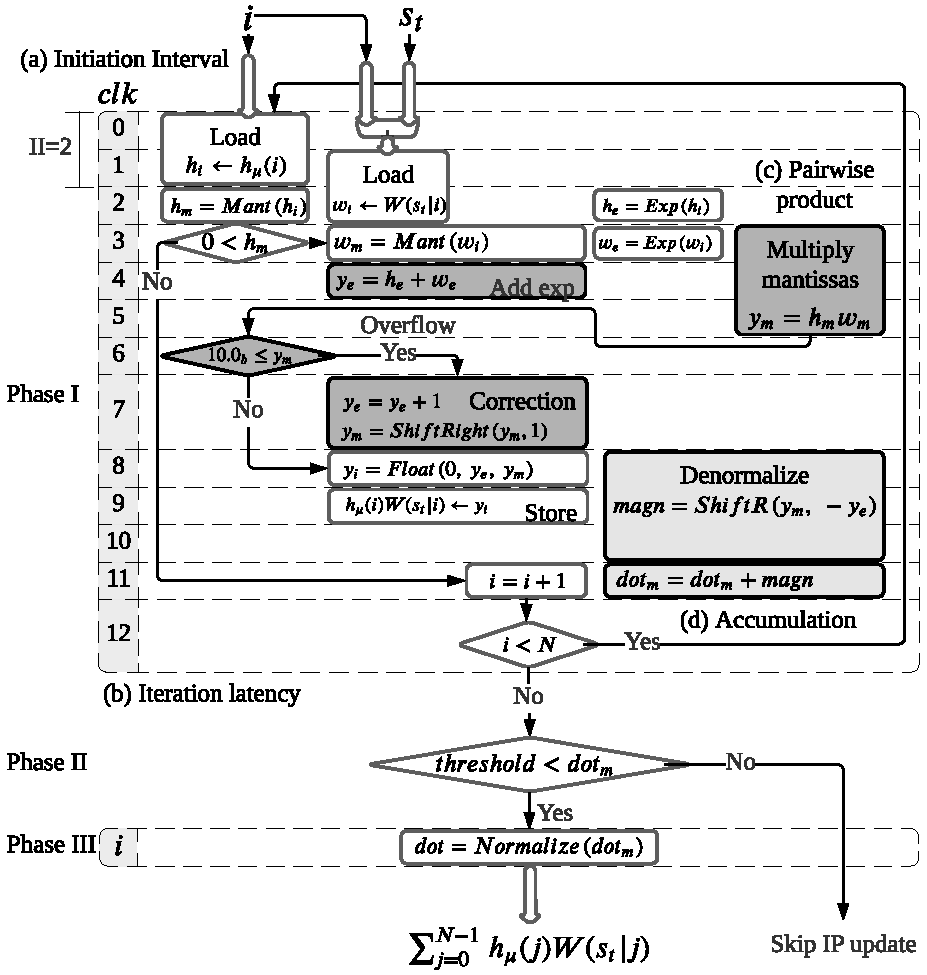
\includegraphics[width=0.5\textwidth]{../figures/dot_product.pdf}
	\caption{Dot-product hardware module with hybrid custom floating-point approximation, (a) exhibits the initiation interval of 2 clock cycles, (b) presents the iteration latency of 13 clock cycles, (c) shows the pairwise product blocks in dark-gray, and (d) illustrates the accumulation blocks in light-gray.}
	\label{fig:dot_product_custom}
\end{figure}

\begin{figure}[t!]
	\centering
	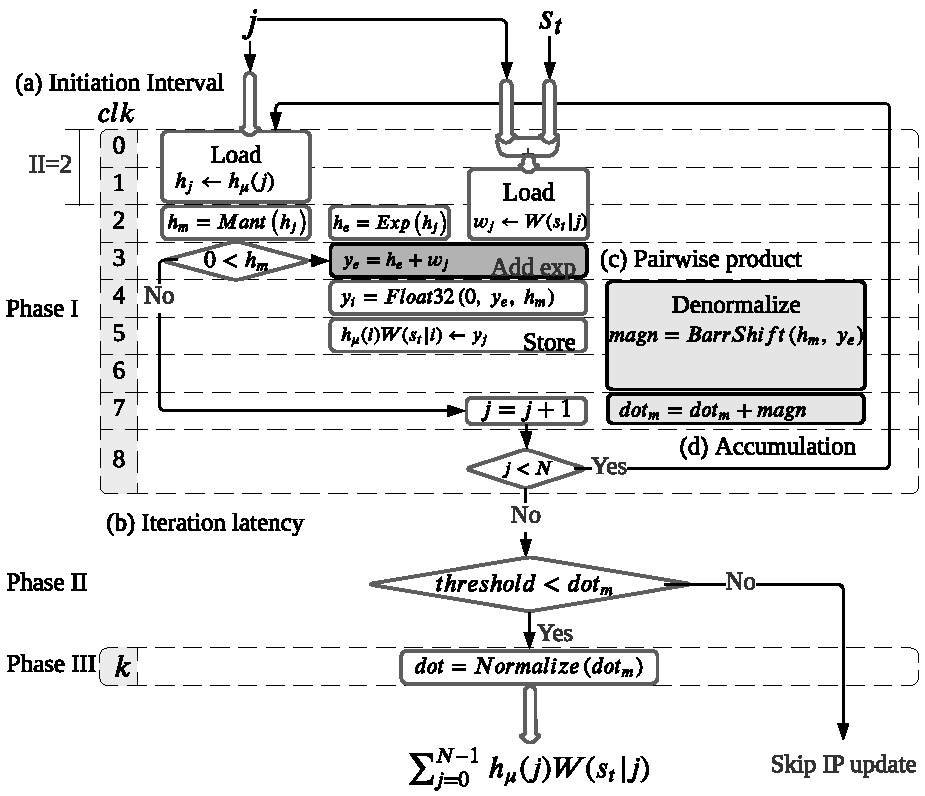
\includegraphics[width=0.5\textwidth]{../figures/dot_product_log.pdf}
	\caption{Dot-product hardware module with hybrid logarithmic approximation, (a) exhibits the initiation interval of 2 clock cycles, (b) presents the iteration latency of 9 clock cycles, (c) shows the pairwise product block in dark-gray, and (d) illustrates the accumulation blocks in light-gray.}
	\label{fig:dot_product_log}
\end{figure}



\section{Experimental results}
\label{sec:experimental_results}
The proposed architecture is demonstrated on a Xilinx Zynq-7020. This device integrates a dual ARM Cortex-A9 based processing system (PS) and programmable logic (PL) equivalent to Xilinx Artix-7 (FPGA) in a single chip \cite{xilinx2015zynq}. The Zynq-7020 architecture conveniently maps the custom logic and software in the PL and PS respectively as an embedded system.

In this platform, we implement the proposed hardware architecture to deploy an SbS network structure for MNIST classification task as shown in \fig{fig:sbs_network}. The training of the SbS model is performed in Matlab and the resulting synaptic weight matrices are deployed on the embedded system. The SbS network is built as a sequential model using the API from the SbS embedded software framework \cite{nevarez2020accelerator}, where the computation of the network is distributed among the hardware processing units and the CPU.

For the evaluation of our approach, we elaborate a design exploration reviewing the computational latency, inference accuracy, noise robustness, resource utilization, and power dissipation. First, we benchmark the performance of SbS network simulation using standard floating-point computation on CPU, and then hardware processing units. Afterwards, we evaluate our dot-product architecture addressing a design exploration using custom floating-point, and then logarithmic computation. Finally, we present a comparison table of the given results.

\begin{figure}[!h]
	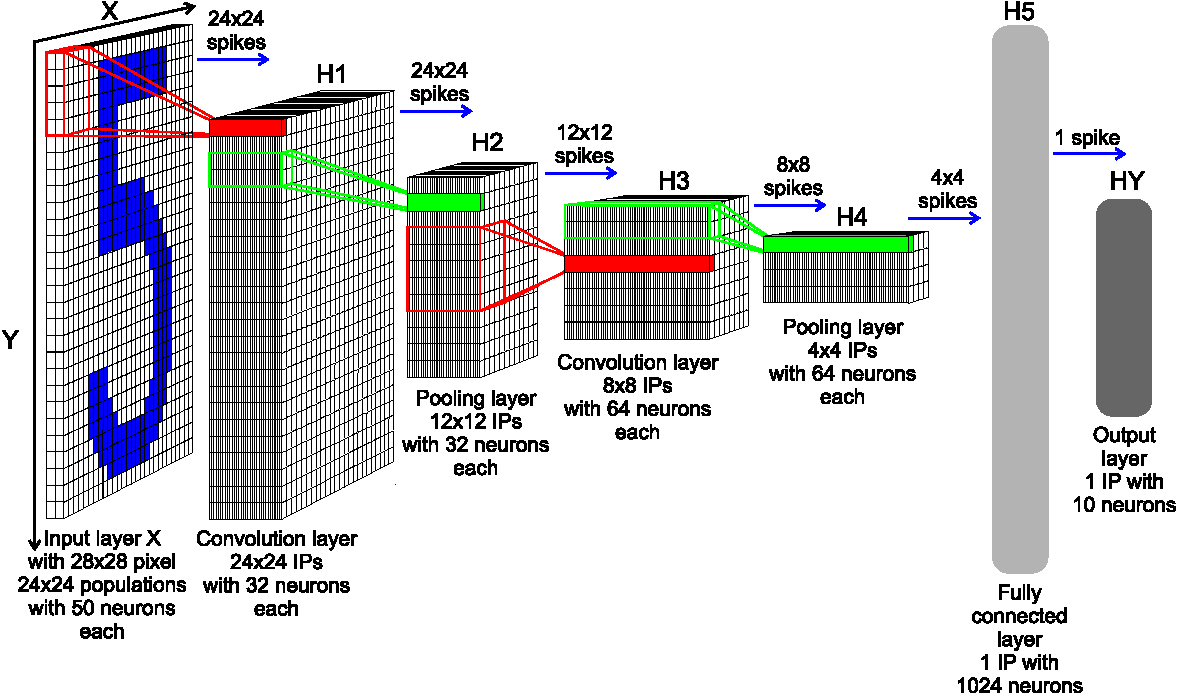
\includegraphics[width=\columnwidth]{../figures/sbs_network.pdf}
	\caption{SbS network structure for MNIST classification task.
		Input \emph{X}: Input layer with $28\times28$ normalization modules for $28\times28$ input pixel. From this layer spikes are send to layer \emph{H1}. \emph{H1}: Convolution layer \emph{H1} with $24\times24$ IPs with $32$ neurons each. Every IP processes the spikes from $5\times5$ spatial patches of the input pattern ($x$ and $y$ stride is $1$). \emph{H2}: $2\times2$ pooling layer \emph{H2} ($x$ and $y$ stride is $2$) with $12\times12$ IPs with $32$ neurons each. The weights between \emph{H1} and \emph{H2} are not learned but set to a fixed weight matrix that creates a competition between the \emph{32} features of \emph{H1}. \emph{H3}: $5\times5$ convolution layer \emph{H3} ($x$ and $y$ stride is $1$) with $8\times8$ IPs. Similar to \emph{H1} but with $64$ neuron  	for each IP. \emph{H4}: $2\times2$ pooling layer \emph{H4} ($x$ and $y$ stride is $2$) with $4\times4$ IPs with $64$ neurons each. This layer is similar to layer \emph{H2}. \emph{H5}: Fully connected layer \emph{H5}. $1,024$ neurons in one big IP which are fully connected to layer \emph{H4} and output layer \emph{HY}. \emph{HY}: Output layer \emph{HY} with $10$ neurons for the $10$ types of digits. selected.}\label{fig:sbs_network}
\end{figure}



\subsection{Performance benchmark}
\subsubsection{Benchmark on CPU}

We examine the performance of the CPU for SbS network simulation with no hardware coprocessing. In this case, the embedded software builds the SbS network as a sequential model mapping the entire computation to the CPU (ARM Cortex-A9) at 666 MHz and a power dissipation of $520 mW$.

The SbS network computation on the CPU achieves a latency of $34.279 ms$ per spike with an accuracy of 99.3\% correct classification on the $10,000$ image test set at $1000$ spikes. The latency and schedule of the SbS network computation are displayed in \Tab{tab:latency_sw} and \fig{fig:latency_sw} respectively.

\begin{table}[!t]\centering
	\caption{Computation on CPU.}\label{tab:latency_sw}
	\scriptsize
\begin{tabular}{lrr}\toprule
	\textbf{Layer} &\textbf{Latency (ms)} \\\midrule
	HX\_IN &1.184 \\
	H1\_CONV &4.865 \\
	H2\_POOL &3.656 \\
	H3\_CONV &20.643 \\
	H4\_POOL &0.828 \\
	H5\_FC &3.099 \\
	HY\_OUT &0.004 \\
		
	TOTAL &34.279 \\
	\bottomrule
\end{tabular}
\end{table}

\begin{figure}[t!]
	\centering
	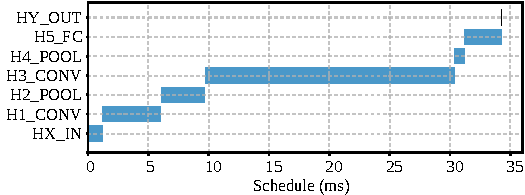
\includegraphics[width=1\columnwidth]{../figures/latency_sw.pdf}
	\caption{Computation on CPU.}
	\label{fig:latency_sw}
\end{figure}

\subsubsection{Benchmark on processing units using standard floating-point}
To benchmark the computation on hardware PUs using standard floating-point, we implement the system architecture shown in \fig{fig:hw_sbs_8_pu}. In this case, the embedded software builds the SbS network as a sequential model mapping the network computation to the hardware processing units at 200 MHz as clock frequency.

\begin{figure}[h!]
	\centering
	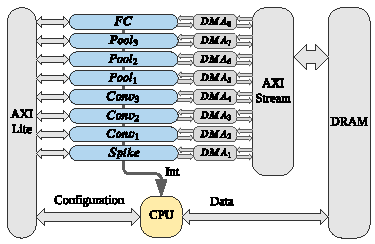
\includegraphics[width=0.5\textwidth]{../figures/sbs_hw_experimental.pdf}
	\caption{System overview of the proposed architecture with 8 processing units.}
	\label{fig:hw_sbs_8_pu}
\end{figure}

In this deployment, it is distributed the computation workload of \emph{H2\_POOL} and \emph{H3\_CONV} among two PUs each one, since these are the heaviest pooling and convolution layers respectively. The output layer \emph{HY\_OUT} is fully processed by the CPU, since it is the lightest one. The hardware mapping and the computation schedule of this deployment are displayed in \Tab{tab:latency_fp} and \fig{fig:latency_pu_fp}.

\begin{table}[!ht]\centering
	\caption{Performance of processing units using standard floating-point computation.}\label{tab:latency_fp}
	\scriptsize
	\begin{tabular}{llrrrrrr}\toprule
		\multicolumn{2}{c}{\textbf{Hardware mapping}} & &\multicolumn{4}{c}{\textbf{Computation schedule (ms)}} \\\cmidrule{1-2}\cmidrule{4-7}
		\textbf{Layer} &\textbf{PU} & &$t_s$ &$t_{CPU}$ &$t_{PU}$ &$t_f$ \\\midrule
		HX\_IN &Spike & &0 &0.056 &0.370 &0.426 \\
		H1\_CONV &Conv1 & &0.058 &0.598 &2.002 &2.658 \\
		\multirow{2}{*}{H2\_POOL}
		&Pool1 & &0.658 &0.126 &1.091 &1.875 \\
		&Pool2 & &0.785 &0.125 &1.075 &1.985 \\
		\multirow{2}{*}{H3\_CONV} 
		&Conv2 & &0.911 &0.280 &3.183 &4.374 \\
		&Conv3 & &1.193 &0.279 &3.176 &4.648 \\
		H4\_POOL &Pool3 & &1.473 &0.037 &0.481 &1.991 \\
		H5\_FC &FC & &1.512 &0.101 &1.118 &2.731 \\
		HY\_OUT &CPU & &1.615 &0.004 &0 &1.619 \\
		\bottomrule
	\end{tabular}
\end{table}

\begin{figure}[!ht]
	\centering
	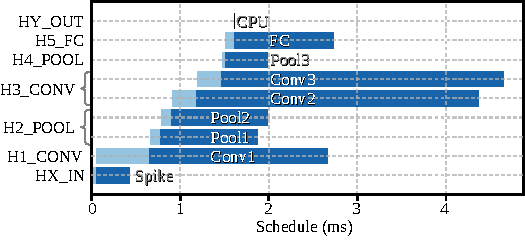
\includegraphics[width=1\columnwidth]{../figures/latency_pu_fp.pdf}
	\caption{Performance of processing units using standard floating-point computation.}
	\label{fig:latency_pu_fp}
\end{figure}

In the computation schedule, the following terms are defined: $t_s(n)$ as the start time of the layer (as a computation node) $n\in L$ where $L$ represents the set of layers, $t_{CPU}(n)$ as the CPU preprocessing time, $t_{PU}(n)$ as the PU latency, and $t_f(n)$ as the finish time. The $t_{CPU}(n)$ is the period of time in which the CPU writes a DRAM buffer with $h_\mu$ (neuron vector) of the current processing layer and $S_t$ (spike vector) from its preceding layer, this buffer is streamed to the PU via DMA.

The total execution time of the CPU is defined by \equ{eq:time_cpu}. In a cyclic inference, the execution time of the network computation is the longest path among the processing units including the CPU, this is denoted as the latency of an spike cycle, and it is defined by \equ{eq:time_spike}. The total execution time of the network computation is the latest finish time defined by \equ{eq:time_finish}.

\begin{figure}[h!]
	\centering
	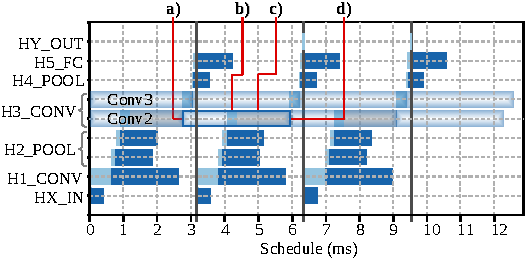
\includegraphics[width=1\columnwidth]{../figures/latency_fp_cycle.pdf}
	\caption{Performance bottleneck of cyclic computation on processing units using standard floating-point. a) Illustrates the starting of $t_{PU}$ of \emph{Conv2} on a previous computation cycle. b) Illustrates $t_{CPU}$ of \emph{Conv2} on the current computation cycle. c) Illustrates the CPU waiting time (in gray color) for \emph{Conv2} as a busy resource (awaiting for \emph{Conv2} interruption). d) Illustrates the $t_{f}$ from the previous computation cycle, and the starting of $t_{PU}$ on the current computation cycle (\emph{Conv2} interruption on completion, and start current computation cycle).}
	\label{fig:latency_pu_fp_cycle}
\end{figure}

\begin{eqnarray} \label{eq:time_cpu}
T_{CPU} = \sum_{n\in L} t_{CPU}(n)
\end{eqnarray}

\begin{eqnarray} \label{eq:time_pu}
T_{PU} = \max_{n\in L}(t_{PU}(n))
\end{eqnarray}

\begin{eqnarray} \label{eq:time_spike}
T_{SC} =
\begin{cases}
T_{PU}, & \text{if}\ T_{CPU}\le T_{PU} \\
T_{CPU}, & \text{otherwise}
\end{cases}
\end{eqnarray}

\begin{eqnarray} \label{eq:time_finish}
T_{f} = \max_{n\in L}(t_{f}(n))
\end{eqnarray}

As the heaviest layer, the computational workload of \emph{H3\_CONV} is evenly partitioned among two PUs: \emph{Conv2} and \emph{Conv3}. However, in the cyclic schedule, \emph{Conv2} causes the performance bottleneck as shown in \fig{fig:latency_pu_fp_cycle}. In this case, the CPU has to await for \emph{Conv2} to finish the computation of the previous cycle in order to start the current computation cycle. Applying \equ{eq:time_spike}, we obtain a latency of 3.183 ms per spike cycle.

This deployment achieves an accuracy of $98.98\%$ correct classification on the $10,000$ image test set at $1000$ spikes. Furthermore, the noise robustness is measured using input patterns with positive additive equidistributed random noise up to $55\%$ of amplitude as shown in \fig{fig:accuracy_vs_noise_pu_fp}. The post-implementation resource utilization and power dissipation are shown in \Tab{tab:resource_fp} and \Tab{tab:power_fp}, respectively.

Each \emph{Conv} PU instantiates a BRAM stationary weight matrix of $52,000$ entries to store $W\in\mathbb{R}^{5\times 5\times 2\times 32}$ and $W\in\mathbb{R}^{5\times 5\times 32\times 64}$ for \emph{H1\_CONV} and \emph{H3\_CONV}, respectively. In order to reduce BRAM utilization, we use a custom floating-point representation composed of 4-exponent and 4-bit mantissa. Each 8-bit entry is promoted to its standard floating-point representation for the dot-product computation. The methodology to find the appropriate bit width parameters for custom floating-point representation is presented in the next section.

\begin{table}[!h]\centering
	\caption{Resource utilization of processing units using standard floating-point.}\label{tab:resource_fp}
	\scriptsize
	\begin{tabular}{lrrrrrr}\toprule
		\textbf{PU} & &\textbf{LUT} &\textbf{FF} &\textbf{DSP} &\textbf{BRAM 18K} \\\midrule
		Spike & &2,640 &4,903 &2 &2 \\
		Conv & &2,765 &4,366 &19 &37 \\
		Pool & &2,273 &3,762 &5 &3 \\
		FC & &2,649 &4,189 &8 &9 \\
		\bottomrule
	\end{tabular}
\end{table}

\begin{table}[!h]\centering
	\caption{Power dissipation of processing units using standard floating-point.}\label{tab:power_fp}
	\scriptsize
	\begin{tabular}{lrr}\toprule
		\textbf{PU} &\textbf{Power (mW)} \\\midrule
		Spike &38 \\
		Conv &89 \\
		Pool &59 \\
		FC &66 \\
		CPU &520 \\
		\bottomrule
	\end{tabular}
\end{table}

\begin{figure}[h!]
	\centering
	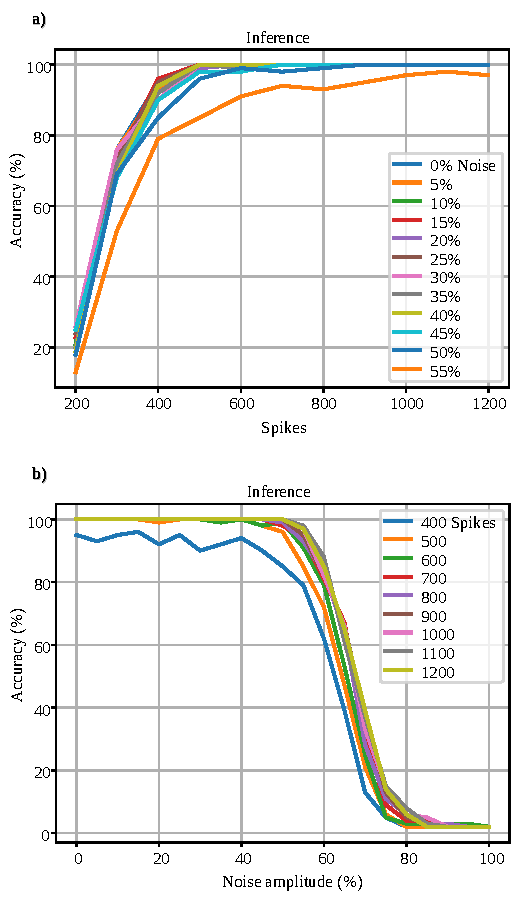
\includegraphics[width=1\columnwidth]{../figures/accuracy_vs_noise_pu_fp.pdf}
	\caption{Benchmark of accuracy and noise robustness of SbS network simulation on hardware PU using standard floating-point computation on 100 images. (a) Illustrates the accuracy vs number of spikes at given noise amplitudes. (b) Illustrates the accuracy vs noise amplitude at given number of spikes.}
	\label{fig:accuracy_vs_noise_pu_fp}
\end{figure}


\subsection{Design exploration for custom floating-point and logarithmic computation}

In this section, we address a design exploration to evaluate our approach for SbS neural network simulation using custom floating-point and logarithmic computation. First, we examine each synaptic weight matrix in order to obtain the minimum requirements for numeric representation and memory storage. Second, we implement the proposed dot-product architecture using the minimal floating-point and logarithmic representation as design parameters. Finally, we evaluate overall performance, inference accuracy, noise robustness, resource utilization, and power dissipation.

\subsubsection{Parameters for numeric representation of synaptic weight matrix}

We obtain the parameters for numeric representation from the $\log_2$-histograms of each synaptic weight matrix as shown in \fig{fig:latency_pu_fp}. Since $0\le W(s_t|j)\le1$ and $\sum_{j=0}^{N-1}W(s_t|j)=1$, the $W$ elements have only negative values in the logarithmic domain; hence, the sign bit is disregarded and the values are stored in its positive version, as stated in Section \ref{Hardware_architecture}. The smallest floating-point entry of $W$ represents the minimum exponent value, as defined by \equ{eq:exp_max}, and the bit width needed for its absolute binary representation is defined by \equ{eq:bits_exp}.

\begin{eqnarray} \label{eq:exp_max}
E_{\min}=\log _2(\min_{\forall i}(W(i)))
\end{eqnarray}

\begin{eqnarray} \label{eq:bits_exp}
N_E=\lceil\log_2(|E_{\min}|)\rceil
\end{eqnarray}

Applying \equ{eq:exp_max} and \equ{eq:bits_exp} to the given SbS network, we obtain $-13$ as the minimum exponent value of the synaptic weights, and 4-bit needed for its absolute binary representation.

As a quality-configurable approximate computing approach, the mantissa bit width is a parameter that is modulated/tuned by the designer. This parameter leverages the builtin error-tolerance of neural networks and performs a trade-off between computation accuracy and synaptic memory footprint. In this publication we present a case study with 1-bit mantissa corresponding to the custom floating-point in the next section.

\begin{figure}[h!]
	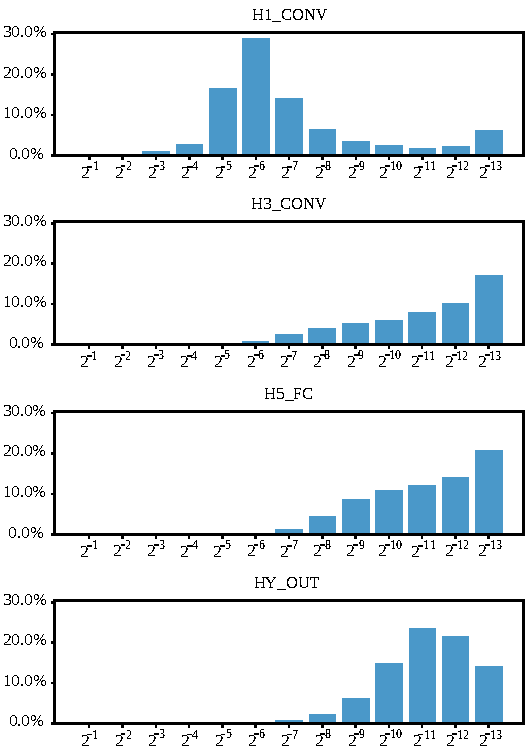
\includegraphics[width=\columnwidth]{../figures/log2_histogram.pdf}
	\caption{$\log_2$-histogram of each synaptic weight matrix showing the percentage of matrix elements with given integer exponent.}\label{fig:log2histogram}
\end{figure}

\subsubsection{Design exploration for dot-product using custom floating-point computation}
For this design exploration, we use a custom floating-point representation composed of 4-bit exponent and 1-bit mantissa for the synaptic weight matrix on the proposed dot-product architecture. In this case, each \emph{Conv} PU instantiates a BRAM stationary weight matrix for $52,000$ entries of 5-bit each one, which is enough to store $W\in\mathbb{R}^{5\times 5\times 2\times 32}$ and $W\in\mathbb{R}^{5\times 5\times 32\times 64}$ for \emph{H1\_CONV} and \emph{H3\_CONV}, respectively. The same dot-product architecture is implemented in \emph{FC} processing unit, however, this does not instantiate BRAM stationary synaptic weight matrix. Instead, \emph{FC} receives neuron and synaptic vectors during performance. The hardware mapping and the computation schedule of this deployment are displayed in \Tab{tab:latency_cfp} and \Fig{fig:latency_pu_cfp_cycle}.

With a reduction from 32-bit ot 5-bit in all the synaptic weight matrices, this design exploration achieves a maximum hardware PU latency of $1.309 ms$ according to \equ{eq:time_pu}, and a CPU latency of $1.673 ms$. Therefore, applying \equ{eq:time_spike}, we obtain a latency of $1.673 ms$ per spike cycle as shown in \Fig{fig:latency_pu_cfp_cycle}. In this case, the cyclic bottleneck is in the CPU performance.

This deployment achieves an accuracy of $98.97\%$ correct classification on the $10,000$ image test set at $1000$ spikes. Furthermore, the noise robustness is shown in \fig{fig:accuracy_vs_noise_pu_cfp}. The post-implementation resource utilization and power dissipation are shown in \Tab{tab:resource_cfp} and \Tab{tab:power_cfp}, respectively.

\begin{table}[t!]\centering
	\caption{Performance of hardware processing units using custom floating-point computation.}\label{tab:latency_cfp}
	\scriptsize
	\begin{tabular}{llrrrrrr}\toprule
		\multicolumn{2}{c}{\textbf{Hardware mapping}} & &\multicolumn{4}{c}{\textbf{Computation schedule (ms)}} \\\cmidrule{1-2}\cmidrule{4-7}
		\textbf{Layer} &\textbf{PU} & &$t_s$ &$t_{CPU}$ &$t_{PU}$ &$t_f$ \\\midrule
		HX\_IN &Spike & &0 &0.055 &0.307 &0.362 \\
		H1\_CONV &Conv1 & &0.057 &0.654 &1.309 &2.020 \\
		\multirow{2}{*}{H2\_POOL} &Pool1 & &0.713 &0.131 &1.098 &1.942 \\
		&Pool2 & &0.845 &0.125 &1.098 &2.068 \\
		\multirow{2}{*}{H3\_CONV} &Conv2 & &0.972 &0.285 &1.199 &2.456 \\
		&Conv3 & &1.258 &0.279 &1.184 &2.721 \\
		H4\_POOL &Pool3 & &1.538 &0.037 &0.484 &2.059 \\
		H5\_FC &FC & &1.577 &0.091 &0.438 &2.106 \\
		HY\_OUT &CPU & &1.669 &0.004 &0 &1.673 \\
		\bottomrule
	\end{tabular}
\end{table}

\begin{figure}[h!]
	\centering
	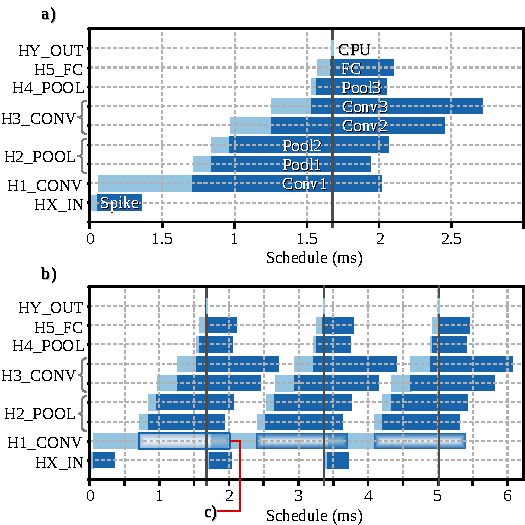
\includegraphics[width=1\columnwidth]{../figures/latency_cfp_cycle.pdf}
	\caption{Performance on processing units using custom floating-point computation. a) Illustrates computation schedule. b) Illustrates cyclic computation schedule. c) Illustrates the performance of \emph{Conv2} from a previous computation cycle during the preprocessing of \emph{H1\_CONV} on the current computation cycle without bottleneck.}
	\label{fig:latency_pu_cfp_cycle}
\end{figure}

\begin{table}[h!]\centering
	\caption{Resource utilization of processing units using custom floating-point.}\label{tab:resource_cfp}
	\scriptsize
	\begin{tabular}{lrrrrrr}\toprule
		\textbf{PU} & &\textbf{LUT} &\textbf{FF} &\textbf{DSP} &\textbf{BRAM 18K} \\\midrule
		Conv & &3,139 &4,850 &19 &25 \\
		FC & &3,265 &5,188 &8 &9 \\
		\bottomrule
	\end{tabular}
\end{table}

\begin{table}[h!]\centering
	\caption{Power dissipation of processing units using custom floating-point.}\label{tab:power_cfp}
	\scriptsize
	\begin{tabular}{lrr}\toprule
		\textbf{PU} &\textbf{Power (mW)} \\\midrule
		Conv &82 \\
		FC &66 \\
		\bottomrule
	\end{tabular}
\end{table}

\begin{figure}[h!]
	\centering
	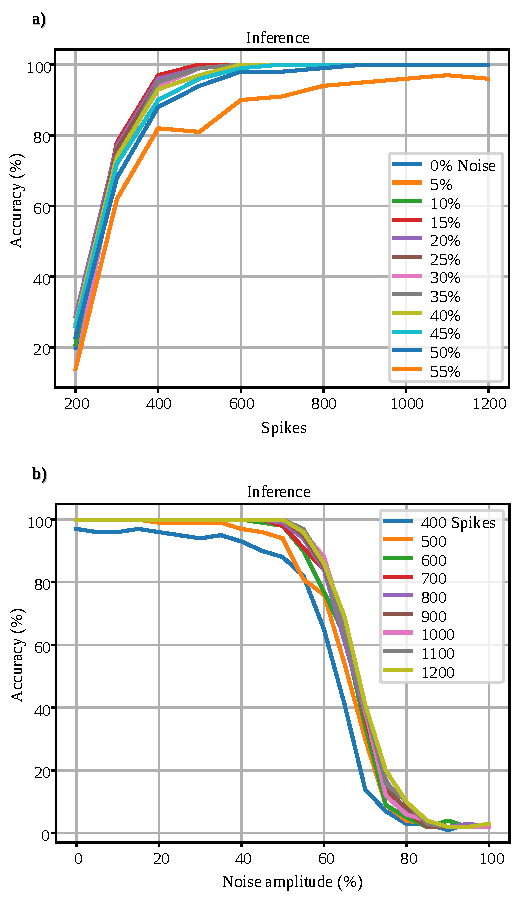
\includegraphics[width=1\columnwidth]{../figures/accuracy_vs_noise_pu_cfp(4-bit-exponent_1-bit-mantissa).pdf}
	\caption{Accuracy and noise robustness of SbS network simulation on hardware PU using custom floating-point computation on 100 images. (a) Illustrates the accuracy vs number of spikes at given noise amplitudes. (b) Illustrates the accuracy vs noise amplitude at given number of spikes.}
	\label{fig:accuracy_vs_noise_pu_cfp}
\end{figure}

\subsubsection{Design exploration for dot-product using logarithmic computation}
For this design exploration, we use a 4-bit integer exponent for logarithmic representation of the synaptic weight matrix. In this case, each \emph{Conv} processing unit implements the proposed dot-product architecture and a BRAM stationary weight matrix for $52,000$ entries of 4-bit integer each one to store $W\in\mathbb{N}^{5\times 5\times 2\times 32}$ and $W\in\mathbb{N}^{5\times 5\times 32\times 64}$ for \emph{H1\_CONV} and \emph{H3\_CONV}, respectively. The same dot-product architecture is implemented in \emph{FC} processing unit without stationary synaptic weight matrix. The hardware mapping and the computation schedule of this deployment are displayed in \Tab{tab:latency_log} and \Fig{fig:latency_pu_log_cycle}.

With a reduction from 32-bit ot 4-bit in all the synaptic weight matrices, this design exploration achieves a maximum hardware PU latency of $1.271 ms$ according to \equ{eq:time_pu}, and a CPU latency of $1.673 ms$. Therefore, applying \equ{eq:time_spike}, we obtain a latency of $1.673 ms$ per spike cycle as shown in \Fig{fig:latency_pu_log_cycle}. In this case, the cyclic bottleneck is in the CPU performance.

This deployment achieves an accuracy of $98.84\%$ correct classification on the $10,000$ image test set at $1000$ spikes. Furthermore, the noise robustness is shown in \fig{fig:accuracy_vs_noise_pu_cfp}. The post-implementation resource utilization and power dissipation are shown in \Tab{tab:resource_cfp} and \Tab{tab:power_cfp}, respectively.

\begin{table}[t!]\centering
	\caption{Performance of hardware processing units using logarithmic computation.}\label{tab:latency_log}
	\scriptsize
	\begin{tabular}{llrrrrrr}\toprule
		\multicolumn{2}{c}{\textbf{Hardware mapping}} & &\multicolumn{4}{c}{\textbf{Computation schedule (ms)}} \\\cmidrule{1-2}\cmidrule{4-7}
		\textbf{Layer} &\textbf{PU} & &$t_s$ &$t_{CPU}$ &$t_{PU}$ &$t_f$ \\\midrule
		HX\_IN &Spike & &0 &0.055 &0.264 &0.319 \\
		H1\_CONV &Conv1 & &0.057 &0.655 &1.271 &1.983 \\
		\multirow{2}{*}{H2\_POOL} &Pool1 & &0.714 &0.130 &1.074 &1.918 \\
		&Pool2 & &0.845 &0.126 &1.106 &2.077 \\
		\multirow{2}{*}{H3\_CONV} &Conv2 & &0.973 &0.285 &1.179 &2.437 \\
		&Conv3 & &1.258 &0.278 &1.176 &2.712 \\
		H4\_POOL &Pool3 & &1.538 &0.037 &0.488 &2.063 \\
		H5\_FC &FC & &1.577 &0.091 &0.388 &2.056 \\
		HY\_OUT &CPU & &1.669 &0.004 &0 &1.673 \\
		\bottomrule
	\end{tabular}
\end{table}

\begin{figure}[!t]
	\centering
	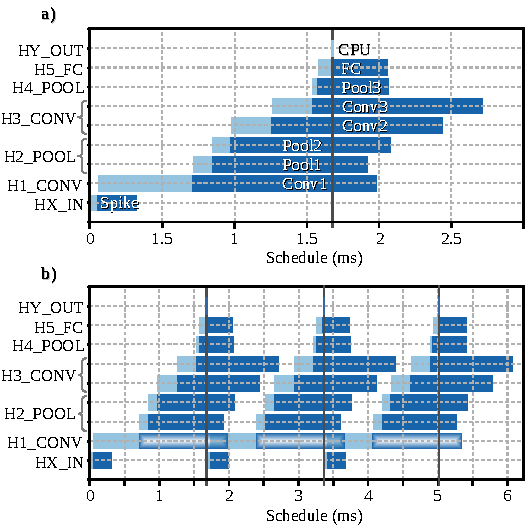
\includegraphics[width=1\columnwidth]{../figures/latency_log_cycle.pdf}
	\caption{Performance of processing units using logarithmic computation. a) Illustrates computation schedule. b) Illustrates cyclic computation schedule.}
	\label{fig:latency_pu_log_cycle}
\end{figure}

\begin{table}[!h]\centering
	\caption{Resource utilization of processing units using logarithmic calculation.}\label{tab:resource_log}
	\scriptsize
	\begin{tabular}{lrrrrrr}\toprule
		\textbf{PU} & &\textbf{LUT} &\textbf{FF} &\textbf{DSP} &\textbf{BRAM 18K} \\\midrule
		Conv & &3,086 &4,804 &19 &21 \\
		FC & &3,046 &4,873 &8 &8 \\
		\bottomrule
	\end{tabular}
\end{table}

\begin{table}[!h]\centering
	\caption{Power dissipation of processing units using logarithmic calculation.}\label{tab:power_log}
	\scriptsize
	\begin{tabular}{lrr}\toprule
		\textbf{PU} &\textbf{Power (W)} \\\midrule
		Conv &78 \\
		FC &66 \\
		\bottomrule
	\end{tabular}
\end{table}

\begin{figure}[h!]
	\centering
	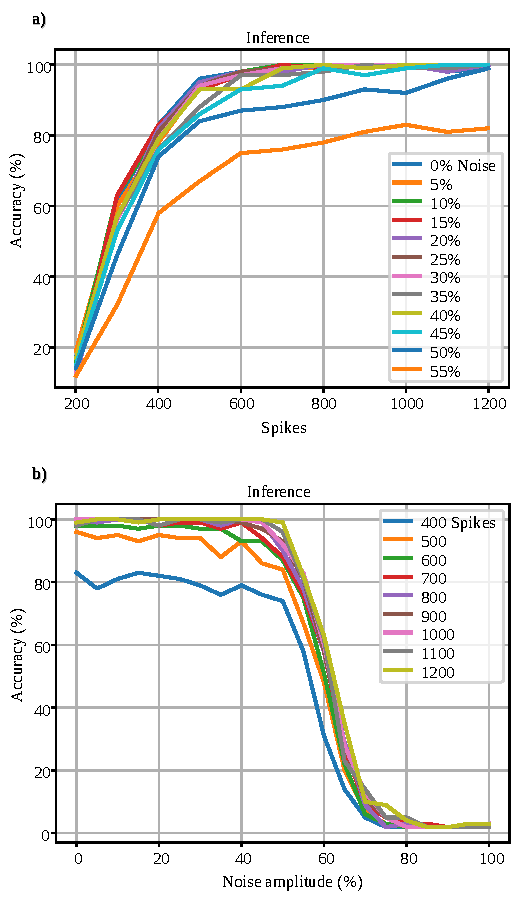
\includegraphics[width=1\columnwidth]{../figures/accuracy_vs_noise_pu_log.pdf}
	\caption{Accuracy and noise robustness of SbS network simulation on hardware PU using logarithmic computation on 100 images. (a) Illustrates the accuracy vs number of spikes at given noise amplitudes. (b) Illustrates the accuracy vs noise amplitude at given number of spikes.}
	\label{fig:accuracy_vs_noise_pu_log}
\end{figure}


\subsection{Results and discussion}
As a benchmark, the SbS network simulation on CPU using 32-bit standard floating-point achieves an accuracy of $99.3\%$ with a latency of spike cycle $T_{SC} = 34.279ms$. As a second benchmark, the network simulation on processing units using 8-bit custom floating-point (4-bit exponent, 4-bit mantissa) for synaptic storage and promoted to standard floating-point for computation achieves an accuracy of $98.98\%$ with a latency $T_{SC}=3.183ms$. As the benchmark result, we get a $10.77\times$ latency enhancement and an accuracy degradation of $0.32\%$.

As a demonstration of the proposed dot-product architecture, the SbS network simulation on hardware PUs with synaptic representation using 5-bit custom floating-point (4-bit exponent, 1-bit mantissa) and 4-bit logarithmic (4-bit exponent) achieve $20.49\times$ latency enhancement and accuracy of $98.97\%$ and $98.84\%$, respectively. As a result, we obtain an accuracy degradation of $0.33\%$ and $0.46\%$, respectively. Moreover, adding 50\% of noise amplitude to the input images, the SbS network simulation presents an accuracy degradation of $0.67\%$ and $4.08\%$, respectively. Regarding resource utilization and power dissipation, the \emph{Conv} processing units present up to $43.24\%$ of BRAM reduction, and $12.35\%$ of energy efficiency improvement over the standard floating-point implementation. The experimental results of the design exploration are summarized in \Tab{tab:results}.

\begin{table*}[!t]
	\begin{threeparttable}
		\centering
		\caption{Experimental results of design exploration.}\label{tab:results}
		\scriptsize
		\begin{tabular}{lrrrrrrrrrrrrrrr}\toprule
			\multirow{2}{*}{\textbf{Implementation}} &\multirow{2}{*}{\textbf{PU}} &\multicolumn{4}{c}{\textbf{Post-implementation resource utilization}} & &\multirow{2}{*}{\textbf{Power (mW)}} & &\multicolumn{2}{c}{\textbf{Latency}} & &\multicolumn{3}{c}{\textbf{Accuracy (\%)\tnote{e}}} \\\cmidrule{3-6}\cmidrule{10-11}\cmidrule{13-15}
			& &\textbf{LUT} &\textbf{FF} &\textbf{DSP} &\textbf{BRAM 18K} & & & &$T_{SC}$ (ms) &\textbf{Gain\tnote{d}} & &\textbf{Noise 0\%} &\textbf{25\%} &\textbf{50\%} \\\midrule
			\multirow{2}{*}{Standard floating-point\tnote{a}} &Conv &2,765 &4,366 &19 &37 & &89 & &\multirow{2}{*}{3.183} &\multirow{2}{*}{10.77x} & &\multirow{2}{*}{98.98} &\multirow{2}{*}{98.96} &\multirow{2}{*}{98.63} \\
			&FC &2,649 &4,189 &8 &9 & &66 & & & & & & & \\
			& & & & & & & & & & & & & & \\
			\multirow{2}{*}{Custom floating-point\tnote{b}} &Conv &3,139 &4,850 &19 &25 & &82 & &\multirow{2}{*}{1.673} &\multirow{2}{*}{20.49x} & &\multirow{2}{*}{98.97} &\multirow{2}{*}{98.94} &\multirow{2}{*}{98.47} \\
			&FC &3,265 &5,188 &8 &9 & &66 & & & & & & & \\
			& & & & & & & & & & & & & & \\
			\multirow{2}{*}{Logarithmic\tnote{c}} &Conv &3,086 &4,804 &19 &21 & &78 & &\multirow{2}{*}{1.673} &\multirow{2}{*}{20.49x} & &\multirow{2}{*}{98.84} &\multirow{2}{*}{98.83} &\multirow{2}{*}{95.22} \\
			&FC &3,046 &4,873 &8 &8 & &66 & & & & & & & \\
			\bottomrule
		\end{tabular}
		\begin{tablenotes}
			\scriptsize
			\item[a] Synaptic storage composed of 4-bit exponent and 4-bit mantissa. For dot-product computation, each entry is promoted to its standard floating-point representation.
			\item[b] Synaptic storage composed of 4-bit exponent and 1-bit mantissa.
			\item[c] Synaptic storage composed of 4-bit exponent.
			\item[d] Latency gain with respect to the CPU computation ($T_{SC} = 34.279 ms$).
			\item[e] Accuracy on 10,000 image test set at 1000 spikes.
		\end{tablenotes}
	\end{threeparttable}
\end{table*}
\section{Conclusions}
\label{sec:conclusions}
In this publication, we accelerate SbS neural networks with a dot-product functional unit based on approximate computing. This approach reduces computational latency, memory footprint, and power dissipation while preserving accuracy and noise robustness. Additionally, the proposed design is compatible with standard floating-point and adaptable as a building block for other error-resilient applications.

We demonstrate our approach addressing a design exploration flow on a Xilinx Zynq-7020 with a deployment of NMIST classification task, this implementation achieves up to $20.49\times$ latency enhancement, $8\times$ synaptic memory footprint reduction, less than $0.5\%$ of accuracy degradation, with a $12.35\%$ of energy efficiency improvement over the standard floating-point hardware implementation. Furthermore, with positive additive uniformly distributed noise at $50\%$ of amplitude on the input image, the SbS network simulation presents an accuracy degradation of less than $5\%$. As application-specific quality metric, the resulting noise robustness demonstrates a sufficient QoR for minimal impact on the overall accuracy of the neural network using the proposed approach. These results suggest available room for further and more aggressive approximation techniques.

In conclusion, based on the relaxed need for fully accurate or deterministic computation of SbS neural networks, approximate computing techniques allow substantial enhancement in processing efficiency with moderated accuracy degradation.

\section * {Acknowledgments}\label{sec:Ack}
This work is funded by the \textit{Consejo Nacional de Ciencia y Tecnologia -- CONACYT} (the Mexican National Council for Science and Technology).


\bibliographystyle{IEEEtran}
\bibliography{../content/bibliography.bib}

\begin{IEEEbiography}[{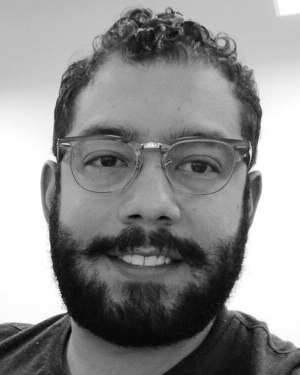
\includegraphics[width=1in,height=1.25in,clip,keepaspectratio]{../biography/yarib_300_375.jpg}}]{Yarib Nevarez} received the B.E. (Hons) degree in electronics from the Durango Institute of Technology, Durango, Mexico, in 2009, and the M.Sc. degree in Embedded Systems Design from the University of Applied Sciences Bremerhaven, Bremen, Germany, in 2017. He is currently pursuing a PhD degree with the Institute of Electrodynamics and Microelectronics, University of Bremen, Germany. His research interest is focused mainly on System-on-Chip architectures and hardware implementation for deep learning accelerators in Embedded Systems.
\\
During his professional experience, he served as a Senior Embedded Software Engineer at Texas Instruments, IBM, Continental Automotive, TOSHIBA, and Carbon Robotics. He has designed and developed software architectures for graphic calculators, automotive systems, robotic drivers, and more.
	
\end{IEEEbiography}

\begin{IEEEbiography}[{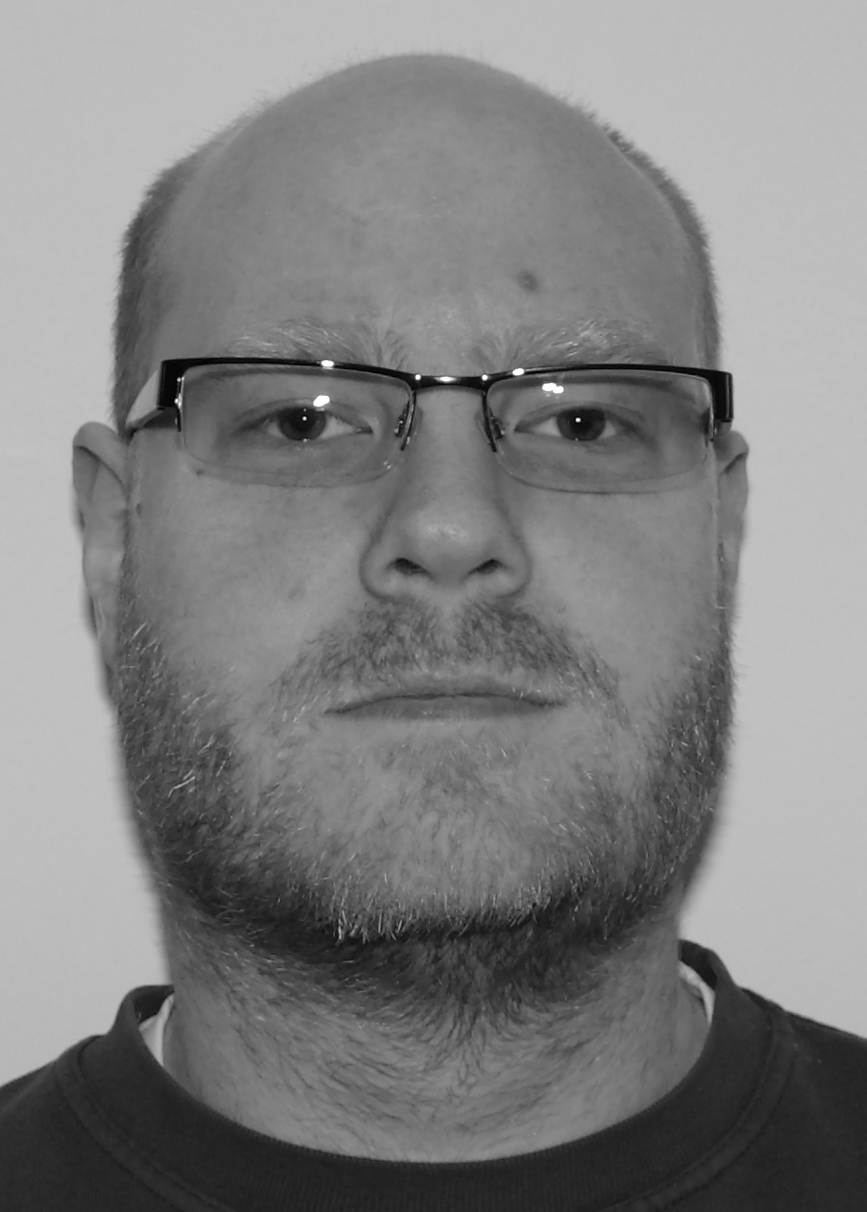
\includegraphics[width=1in,height=1.25in,clip,keepaspectratio]{../biography/Rotermund_David.jpg}}]{David Rotermund} started his scientific career as a chemical technical assistant in 1992 and received a pre-diploma in electrical engineering at the Hochschule Bremen (City University for Applied Science) in 1996. In 2002, he finished his studies of physics at the University of Bremen with a diploma (specialization in neuroscience and solid state physics). In 2007 he received his PhD "Extraction of information from the dynamical activities of neural networks". Among other neuroscience projects, he participated in several project in the field of neuro-prosthetics like the German-Israeli joint project "Models and Experiments towards Adaptive Control of Motor Prostheses" (METACOMP), the research focus Neurotechnology at the University of Bremen, and the Creative Unit "I-See: The artificial eye -- chronic wireless interface to the visual cortex". In the BMBF project KALOMED, where the goal was to design a fully wireless recording system that can be implanted under the skull of an user, he worked as project organizer and hardware/ software/ firmware designer as well as data miner. He will be the co-organizer of the upcoming Era-Net Neuron (a joint Canadian / EU project) for the development of advanced techniques in the field of visual cortex prosthesis. Beside his research in the field of neuro-prosthetics, he is keenly interested in information processing using spiking neuronal networks.
\end{IEEEbiography}

\begin{IEEEbiography}[{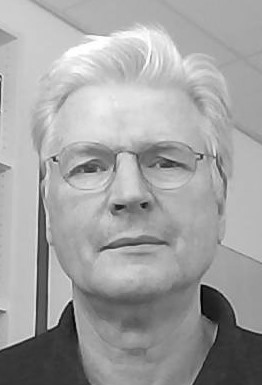
\includegraphics[width=1in,height=1.25in,clip,keepaspectratio]{../biography/Klaus.jpg}}]{Klaus R. Pawelzik}
	received his PhD in the field of Nonlinear Dynamics in
	1990.  From 1991 till March 1998 he was research assistant at several
	well-known institutes in Germany and the US. Since April 1998 he is a
	tenured professor for Theoretical Physics and Theoretical Biology at the
	University of Bremen. He works mainly on topics in Theoretical
	Neuroscience, but also on problems in Neuro-technology and studies
	models of other complex adaptive systems. His many publications
	underline his expertise in these fields. Currently he is the director of
	the Center of Cognitive Sciences at the University of Bremen and has
	raised a number of third-party funds, among them several in the field of
	Neuro-technology. There he recently filed a patent with the title
	"Artificial neural network data processing apparatus and data processing
	method".
\end{IEEEbiography}

\begin{IEEEbiography}[{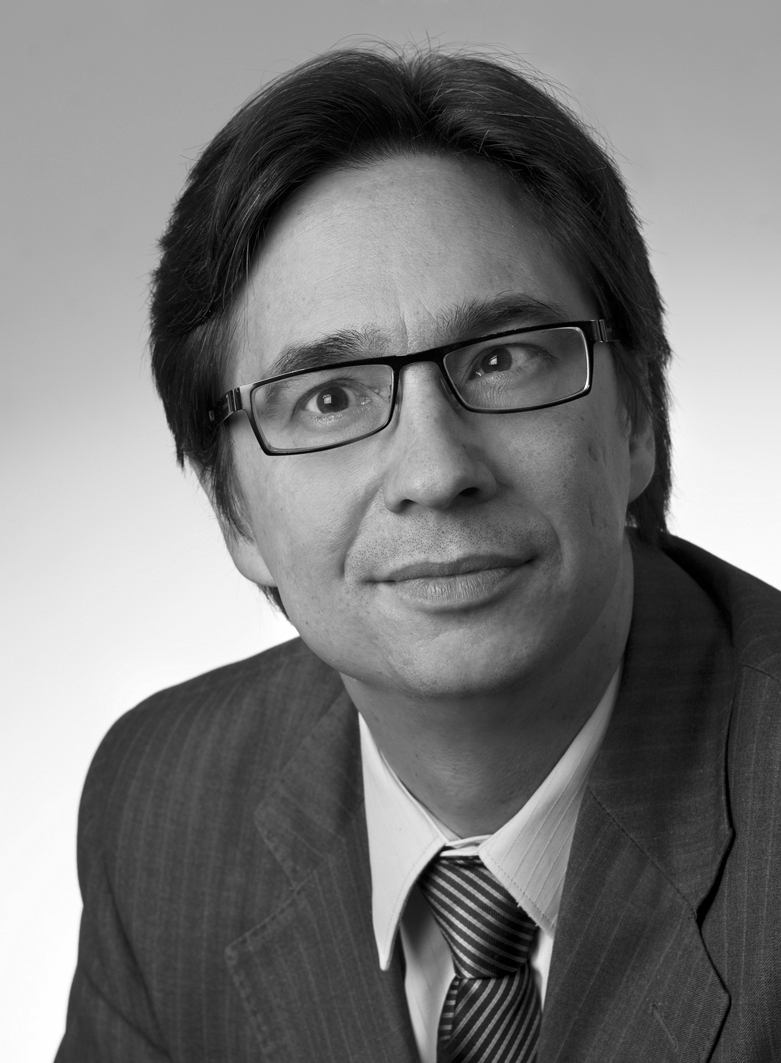
\includegraphics[width=1in,height=1.25in,clip,keepaspectratio]{../biography/Alberto_Garcia-Ortiz.jpg}}]{Alberto Garcia-Ortiz}
    obtained the diploma degree in
    Telecommunication Systems from the Polytechnic University of
    Valencia (Spain) in 1998. After working for two years at Newlogic
    in Austria, he started the Ph.D. at the Institute of
    Microelectronic Systems, Darmstadt University of Technology,
    Germany. In 2003, he received from the Department of Electrical
    Engineering and Information Technology of the university the
    Ph.D. degree with "summa cum laude." From 2003 to 2005, he worked
    as a Senior Hardware Design Engineer at IBM Deutschland
    Development and Research in B{\"o}blingen.  After that he joined the
    start-up AnaFocus (Spain), where he was responsible for the design
    and integration of AnaFocus" next generation Vision
    Systems-on-Chip. He is currently full professor for the chair of
    integrated digital systems at the university of Bremen.
    Dr. Garcia-Ortiz received the "Outstanding dissertation award" in
    2004 from the European Design and Automation Association. In 2005,
    he received from IBM an innovation award for contributions to
    leakage estimation. Two patents are issued with that work. He
    serves as editor of JOLPE and is reviewer of several conferences,
    journals, and European projects. \\
    His interests include low-power
    design and estimation, communication- centric design, SoC
    integration, and variations-aware design. 
\end{IEEEbiography}


\EOD

\end{document}
